\documentclass[11pt,a4paper]{article}

\usepackage[T1]{fontenc}
% Zotero exports some CHI/IUI series fields with a Unicode prime (IUI′15).
\DeclareUnicodeCharacter{2032}{'}
\usepackage[default]{sourceserifpro}
\usepackage{sourcesanspro}
\usepackage[margin=2.2cm]{geometry}
\usepackage{microtype}
\usepackage[table]{xcolor}
\usepackage{caption}
\usepackage{titlesec}
\usepackage{cite}
\usepackage{graphicx}
\usepackage[export]{adjustbox}
\usepackage{tabularx}
\usepackage{xltabular}
\usepackage{array}
\usepackage{booktabs}
\usepackage{float}
\usepackage[section]{placeins}
\renewcommand{\topfraction}{0.92}\renewcommand{\bottomfraction}{0.8}\renewcommand{\textfraction}{0.06}\renewcommand{\floatpagefraction}{0.85}
\usepackage{tikz}
\usetikzlibrary{positioning,arrows.meta,fit,calc,backgrounds}

\definecolor{inkprimary}{HTML}{1A1A19}
\definecolor{inkmuted}{HTML}{52514E}
\definecolor{gridline}{HTML}{E6E5E2}
\definecolor{accent}{HTML}{2A78D6}
\definecolor{warm}{HTML}{D9663A}
\definecolor{failred}{HTML}{B3261E}
\color{inkprimary}

\captionsetup{font=footnotesize}
\titleformat{\section}{\normalfont\sffamily\large\bfseries}{}{0em}{}
\titlespacing*{\section}{0pt}{1.1ex}{0.5ex}
\setlength{\parskip}{0.45ex}

\usepackage[hidelinks]{hyperref}
\hypersetup{
  pdftitle  = {Your Camera Roll, Your Story: Selection and Storytelling with Adjustable AI Help},
  pdfauthor = {Kashyap Shankar Iyer},
}

% Figure images are copies of phone screenshots with personal photos, so they live in figures/,
% which is git-ignored, and the built PDF is not committed either.
\graphicspath{{figures/}}

% Counted words: the abstract, and the main report from the Scope section to the end of the
% Compromises section, including the rationale table's text. Figures, storyboards, captions, the
% title block, repository links and references are excluded by the brief and wrapped in
% TC:ignore. The table is an xltabular, so texcount counts its text with the section.
\newcommand{\abstractcount}{281}
\newcommand{\maincount}{1076}
\newcommand{\totalcount}{1357}
\newcommand{\repo}{\href{https://github.com/kashyap-17/inkreel}{github.com/kashyap-17/inkreel}}
\newcommand{\commit}{\href{https://github.com/kashyap-17/inkreel/tree/a2-final}{tag \texttt{a2-final}}}

% A storyboard frame: an image cropped to its useful part (trim = left bottom right top, in px),
% with a number, who acts (P person, S system) and a short label.
\newcommand{\frameimg}[4]{%
  \begin{minipage}[t]{#1}\centering
  \includegraphics[width=\linewidth,trim=#2,clip,valign=t]{#3}\\[2pt]
  \parbox[t]{\linewidth}{\raggedright\sffamily\scriptsize #4}%
  \end{minipage}}

\newcolumntype{L}[1]{>{\raggedright\arraybackslash}p{#1}}
\newcolumntype{Y}{>{\raggedright\arraybackslash}X}

\begin{document}

%TC:ignore
\begin{center}
  {\sffamily\Large\bfseries Your Camera Roll, Your Story:\\
  Selection and Storytelling with Adjustable AI Help}\\[1ex]
  {\sffamily Kashyap Shankar Iyer (3087617) \quad·\quad Intelligent Interactive Systems,
  Assignment~2: Project Report}\\[0.6ex]
  {\sffamily\bfseries Word count: \totalcount\ (abstract \abstractcount, main report \maincount)}\\[0.4ex]
  {\sffamily\small Repository and README: \repo \quad·\quad submitted commit \commit}
\end{center}
%TC:endignore

\section{Abstract}

From an album of photos, say from a holiday, many people want to share a few on social media,
with words that sound like them. Existing AI tools start from the photos and write the captions
from scratch, so people rarely feel the words are their own, and those who already know what they
want to say must still find the photos themselves. Inkreel reverses the order: the person starts
with their words, in full or as a few notes, and Inkreel finds the photos in their album that fit, with a short reason
for each match, then builds a carousel and caption for social media, such as Instagram.

I built Inkreel as a mobile web app (Next.js, with Google's Gemini models) and tested
it on my phone with my own photos. It has two writing modes. In ``I have writing'', the
person's words are never changed: the caption is the writing exactly as typed. In ``Write with
Inkreel'', four short prompts (a moment, a place or thing, how it felt, anything else) guide the
person to note what made it theirs, and the AI drafts lines from those notes; each line
shows which notes it came from, their own words are highlighted, and any line can be
edited, dropped or redrafted. In both modes, an LLM turns each line into photo searches,
image embeddings score the photos, code picks a photo for each part, and
the LLM checks each pick and writes its reason. The person can swap, add or remove photos before sharing.

Current scope: the core loop is deployed and tested. Planned: text on the
images, and a study of match quality and ownership with other people.

\section{Design rationale}

Table~\ref{tab:rationale} lists the main choices.

{\footnotesize\renewcommand{\arraystretch}{1.18}
\begin{xltabular}{\textwidth}{@{}L{3.4cm}YL{2.95cm}L{1.75cm}@{}}
\caption{Design rationale. Lecture labels: L02 the simplest system that works; L04 feedback
timing; L05 recognition over recall; L06 bounded rationality and anchoring; L08 LLMs generate,
not look up; L11 sources shown, not just cited; L12 confirm what cannot be undone or seen.}\label{tab:rationale}\\
\toprule
\textbf{Design choice} & \textbf{Why it suits the problem} & \textbf{Evidence or reference} & \textbf{Status}\\
\midrule
\endfirsthead
\toprule\multicolumn{4}{@{}l}{\textit{Table 1, continued}}\\
\textbf{Design choice} & \textbf{Why it suits the problem} & \textbf{Evidence or reference} & \textbf{Status}\\
\midrule
\endhead

\textbf{Words first:} the person writes, then adds photos; Inkreel finds photos that fit.
& People also tell photo stories story-first; AI tools serve only photo-first telling.
& Balabanović et al.~\cite{balabanovic_storytelling_2000}; my market check
& Implemented\\
\rowcolor{gridline!45}
\textbf{Words never changed:} code splits them at sentence and line breaks; the caption is the
text as typed.
& Ownership falls as the AI's share rises~\cite{draxler_ai_2024}. A model generates rather than
copies (generation, not lookup, L08), so no model touches this text.
& Unit test: parts rejoin into the exact text. A couplet split in my test: blank lines now
kept.
& Implemented\\
\textbf{A reason and a swap per match:} the reason quotes the line; ``Change photo'' offers the
next picks first.
& Correction must be cheap~\cite{horvitz_principles_1999}. People take the first-ranked
option (bounded rationality, L06), so alternatives are shown; a reason beside the photo is
checked at a glance (shown, not just cited, L11).
& Explanatory debugging~\cite{kulesza_principles_2015}; Guidelines 9 and
11~\cite{amershi_guidelines_2019}
& Implemented\\
\rowcolor{gridline!45}
\textbf{Search, not description:} an LLM turns each line into up to three visual readings;
embeddings score the photos; code picks; the LLM checks only the picks.
& Each photo is embedded once, and feelings need rewording into what a camera sees. The path is
known, so a fixed workflow, not an agent, is the simplest system that works (L02).
& Plain lines once beat the readings, so each line is also searched as written.
& Implemented\\
\textbf{Four labelled thoughts, used as hints:} the AI writes 2--4 lines; named places become
hashtags.
& Labels turn recall into recognition (L05). Notes reused word
for word read as a list.
& I rejected versions 2--8 as reworded answers (Figure~\ref{fig:prompts}).
& Implemented\\
\rowcolor{gridline!45}
\textbf{Provenance per drafted line:} its source thoughts; own words highlighted by code; edit,
drop, draft again.
& Ownership rises with the person's influence over the text~\cite{draxler_ai_2024}. AI
suggestions shift what people
write~\cite{jakesch_co-writing_2023}, so the AI adds no facts. A first draft anchors the edit
(anchoring, L06), so changing it is one tap.
& On my phone: every line showed its sources (Figure~\ref{fig:sb-write})
& Implemented\\
\textbf{Consent once, little data:} small copies without location leave after one consent;
weak photos are set aside, restorable.
& Sending cannot be undone or seen, so Inkreel asks; setting aside is reversible and visible, so it
acts and shows it (L12). Automation and control both stay
high~\cite{shneiderman_human-centered_2022}.
& Consent screen (Figure~\ref{fig:sb-fail})
& Implemented\\
\rowcolor{gridline!45}
\textbf{A wait that keeps moving:} a progress bar with the step and time left; backup requests
for calls that hang.
& Response-time limits of about 0.1, 1 and 10~s (L04, after Miller~\cite{miller_response_1968}); model calls
vary, and the API was often busy (L08).
& Matching took 10 minutes once, now 8~s
& Implemented\\
\textbf{Text on images:} each line placed on its photo.
& Shows which line goes with which photo, which a caption alone hides.
& Captions first, to learn from real posts
& Planned\\
\bottomrule
\end{xltabular}}


\section{System}

Most of the work (Figures~\ref{fig:arch} and~\ref{fig:flow}) is ordinary code on the phone, with no
AI: reading photos, setting weak ones aside,
stacking, scoring and splitting the writing, which keeps it fast, free and testable. The server
holds the API key, checks the invite code and validates every request and reply against a schema,
which guarantees shape, not truth (L09). The AI has three jobs, each one call with a versioned
prompt. Matching depends on two of them: photo vectors and search phrases are made in parallel,
code combines them, and only then does the check see the chosen photos. Each AI output is a
proposal that code checks (the model proposes, the system disposes; L12): a cited thought must
exist, a new place name is flagged, a rejected photo is replaced. A failed call makes the step
that depends on it fall back, never leaving the person stuck.

%TC:ignore
% Figure 1: system diagram. Solid = implemented, dashed = planned, dotted = simulated (tests only).
\begin{figure}[!htbp]
\centering
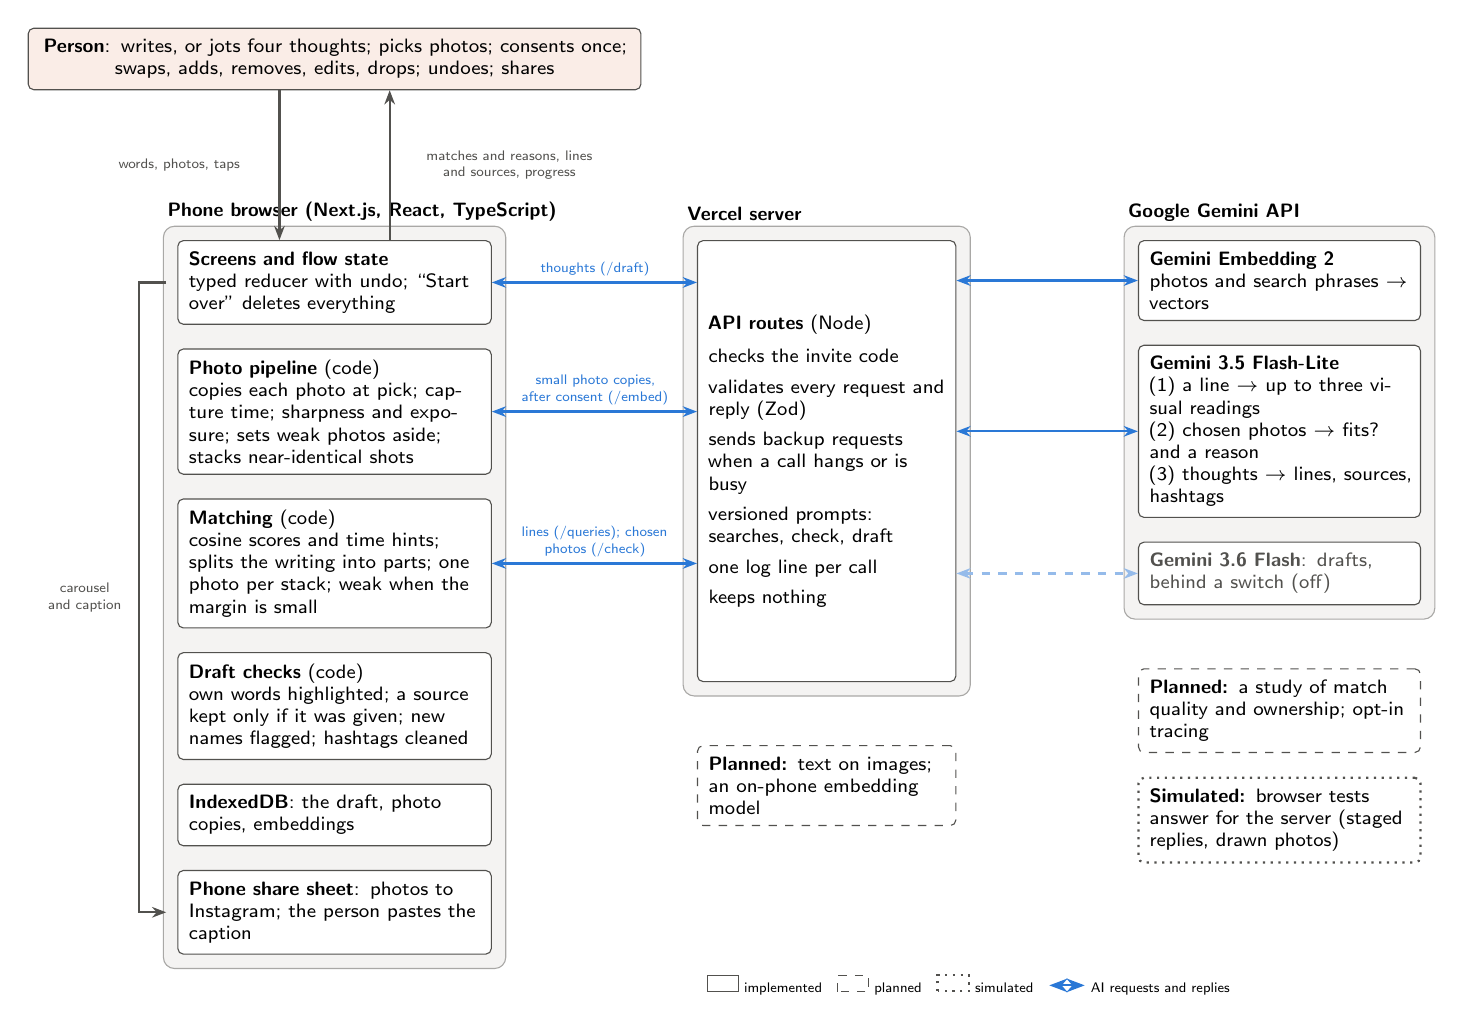
\begin{tikzpicture}[
  font=\sffamily\scriptsize,
  box/.style={draw=inkmuted, rounded corners=2pt, fill=white, text width=#1, align=left, inner sep=4pt},
  box/.default=3.7cm,
  plan/.style={box=#1, dashed},
  plan/.default=3.2cm,
  sim/.style={box=#1, dotted, thick},
  sim/.default=3.5cm,
  zone/.style={draw=inkmuted!50, rounded corners=4pt, fill=gridline!45, inner sep=5pt},
  ztitle/.style={font=\sffamily\scriptsize\bfseries, anchor=south west, inner sep=1.5pt},
  arr/.style={-{Stealth[length=1.8mm]}, inkmuted, thick},
  two/.style={{Stealth[length=1.8mm]}-{Stealth[length=1.8mm]}, accent, thick},
  lab/.style={font=\sffamily\tiny, text width=#1, align=center, inner sep=1pt},
  lab/.default=2.0cm,
  node distance=0.3cm,
]
% ---- Person (top)
\node[box=7.5cm, fill=warm!12, align=center] (person) at (2.0,6.9) {\textbf{Person}: writes, or jots four thoughts; picks photos; consents once;\\swaps, adds, removes, edits, drops; undoes; shares};

% ---- Phone browser (x = 2.0)
\node[box, anchor=north] (ui) at (2.0,4.6) {\textbf{Screens and flow state}\\typed reducer with undo; ``Start over'' deletes everything};
\node[box, below=of ui] (pp) {\textbf{Photo pipeline} (code)\\copies each photo at pick; capture time; sharpness and exposure; sets weak photos aside; stacks near-identical shots};
\node[box, below=of pp] (mt) {\textbf{Matching} (code)\\cosine scores and time hints; splits the writing into parts; one photo per stack; weak when the margin is small};
\node[box, below=of mt] (dc) {\textbf{Draft checks} (code)\\own words highlighted; a source kept only if it was given; new names flagged; hashtags cleaned};
\node[box, below=of dc] (db) {\textbf{IndexedDB}: the draft, photo copies, embeddings};
\node[box, below=of db] (share) {\textbf{Phone share sheet}: photos to Instagram; the person pastes the caption};
\begin{scope}[on background layer]
\node[zone, fit=(ui)(pp)(mt)(dc)(db)(share)] (phone) {};
\end{scope}
\node[ztitle] at (phone.north west) {Phone browser (Next.js, React, TypeScript)};

% ---- Vercel (x = 8.25)
\node[box=3.0cm, anchor=north, minimum height=5.6cm] (api) at (8.25,4.6) {\textbf{API routes} (Node)\\[4pt]
  checks the invite code\\[3pt]
  validates every request and reply (Zod)\\[3pt]
  sends backup requests when a call hangs or is busy\\[3pt]
  versioned prompts: searches, check, draft\\[3pt]
  one log line per call\\[3pt]
  keeps nothing};
\begin{scope}[on background layer]
\node[zone, fit=(api)] (server) {};
\end{scope}
\node[ztitle] at (server.north west) {Vercel server};

% ---- Gemini (x = 14.0)
\node[box=3.3cm, anchor=north] (emb) at (14.0,4.6) {\textbf{Gemini Embedding 2}\\photos and search phrases $\rightarrow$ vectors};
\node[box=3.3cm, below=of emb] (lite) {\textbf{Gemini 3.5 Flash-Lite}\\(1) a line $\rightarrow$ up to three visual readings\\(2) chosen photos $\rightarrow$ fits? and a reason\\(3) thoughts $\rightarrow$ lines, sources, hashtags};
\node[box=3.3cm, below=of lite, text=inkmuted] (flash) {\textbf{Gemini 3.6 Flash}: drafts, behind a switch (off)};
\begin{scope}[on background layer]
\node[zone, fit=(emb)(lite)(flash)] (google) {};
\end{scope}
\node[ztitle] at (google.north west) {Google Gemini API};

% ---- Planned and simulated
\node[plan=3.0cm, below=0.8cm of api] (txt) {\textbf{Planned:} text on images; an on-phone embedding model};
\node[plan=3.3cm, below=0.8cm of flash] (study) {\textbf{Planned:} a study of match quality and ownership; opt-in tracing};
\node[sim=3.3cm, below=of study] (tests) {\textbf{Simulated:} browser tests answer for the server (staged replies, drawn photos)};

% ---- Arrows
\draw[arr] ([xshift=-0.7cm]person.south) -- node[lab=2.3cm, left=2pt] {words, photos, taps} ([xshift=-0.7cm]person.south |- ui.north);
\draw[arr] ([xshift=0.7cm]person.south |- ui.north) -- node[lab=2.8cm, right=2pt] {matches and reasons, lines and sources, progress} ([xshift=0.7cm]person.south);
\draw[two] (ui.east) -- node[lab, above=1pt] {thoughts (/draft)} (ui.east -| api.west);
\draw[two] (pp.east) -- node[lab, above=1pt] {small photo copies, after consent (/embed)} (pp.east -| api.west);
\draw[two] (mt.east) -- node[lab, above=1pt] {lines (/queries); chosen photos (/check)} (mt.east -| api.west);
\draw[two] (emb.west -| api.east) -- (emb.west);
\draw[two] (lite.west -| api.east) -- (lite.west);
\draw[two, dashed, accent!50] (flash.west -| api.east) -- (flash.west);
\draw[arr] ([xshift=-4pt]ui.west) -- ++(-0.35,0) |- node[lab=1.2cm, pos=0.25, left=1pt] {carousel and caption} ([xshift=-4pt]share.west);

% ---- Legend
\node[anchor=north west, font=\sffamily\tiny, align=left] at (6.6,-4.6) {%
  \tikz\draw[inkmuted] (0,0) rectangle (0.4,0.2); implemented\quad
  \tikz\draw[inkmuted, dashed] (0,0) rectangle (0.4,0.2); planned\quad
  \tikz\draw[inkmuted, dotted, thick] (0,0) rectangle (0.4,0.2); simulated\quad
  \tikz\draw[accent, thick, {Stealth}-{Stealth}] (0,0.1) -- (0.45,0.1); AI requests and replies};
\end{tikzpicture}
\caption{System diagram. The screens call the phone's code modules; only the three blue routes
leave the phone. The AI's output is a proposal: code checks and arranges it, and the person
decides.}
\label{fig:arch}
\end{figure}

% Figure 2: the flow as built, with failure paths (red) and the person's changes (blue).
\begin{figure}[p]
\centering
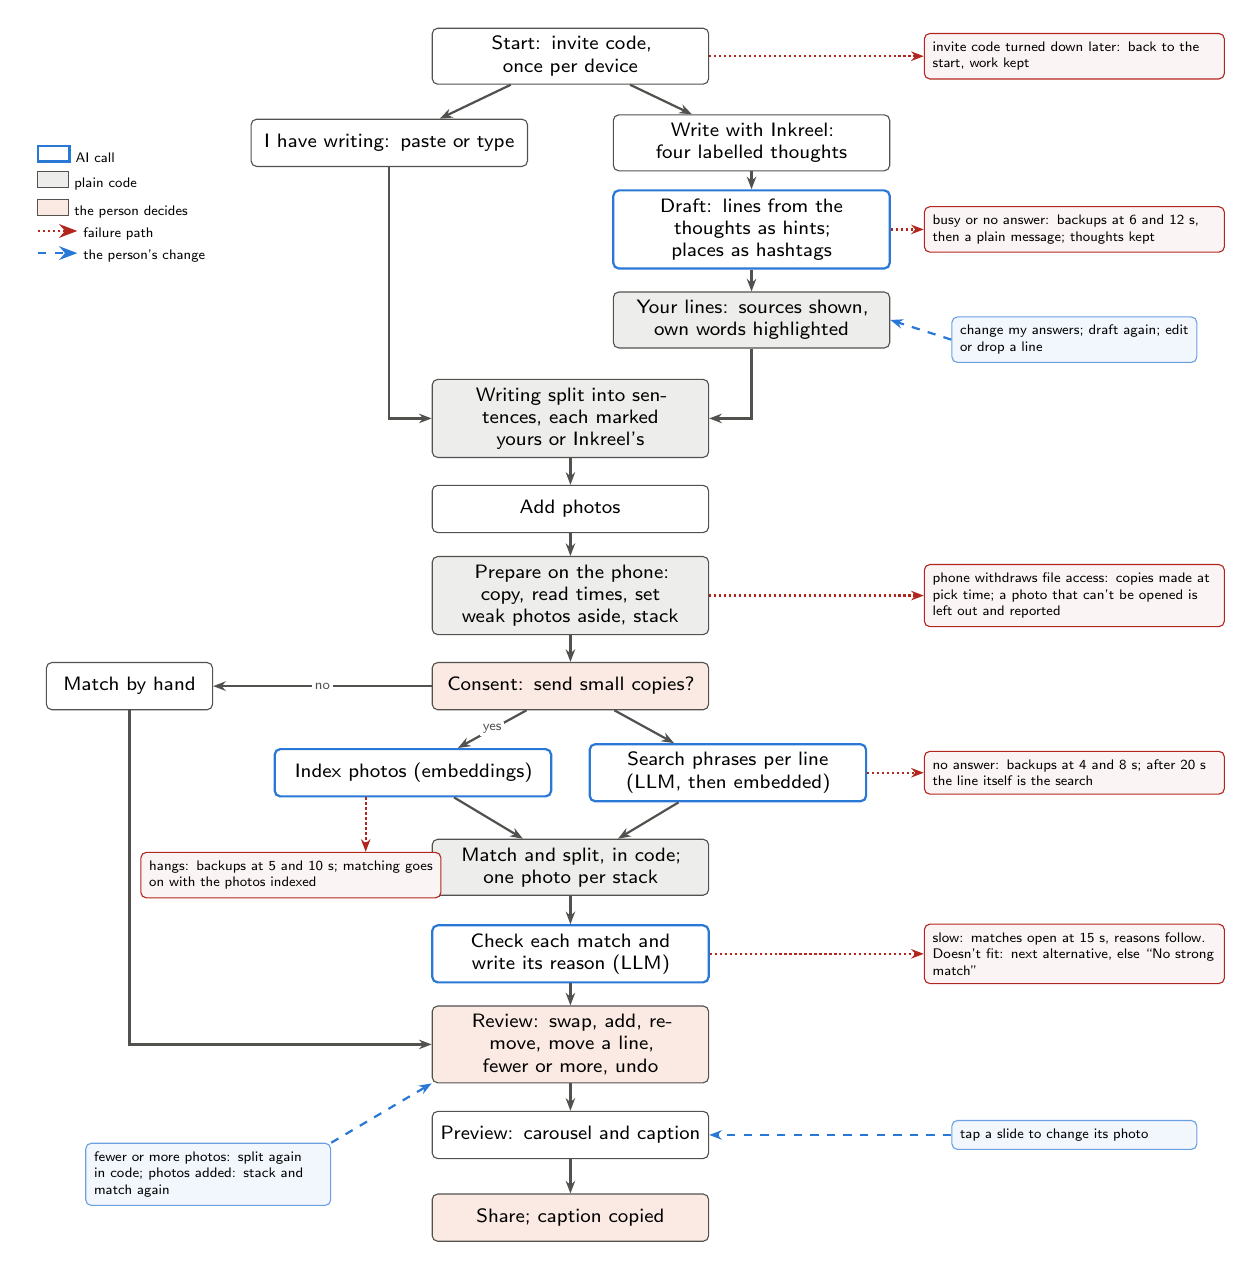
\begin{tikzpicture}[
  font=\sffamily\scriptsize,
  st/.style={draw=inkmuted, rounded corners=2pt, fill=white, text width=3.3cm, align=center, inner sep=3pt, minimum height=0.6cm},
  code/.style={st, fill=gridline!70},
  ai/.style={st, draw=accent, thick},
  dec/.style={st, fill=warm!14},
  fail/.style={draw=failred, rounded corners=2pt, fill=failred!5, text width=3.6cm, align=left, inner sep=3pt, font=\sffamily\tiny},
  user/.style={draw=accent!70, rounded corners=2pt, fill=accent!6, text width=2.9cm, align=left, inner sep=3pt, font=\sffamily\tiny},
  arr/.style={-{Stealth[length=1.6mm]}, inkmuted, thick},
  farr/.style={-{Stealth[length=1.6mm]}, failred, densely dotted, thick},
  uarr/.style={-{Stealth[length=1.6mm]}, accent, dashed, thick},
  tag/.style={font=\sffamily\tiny, fill=white, inner sep=1pt},
]
% main path
\node[st]   (start) at (0,0)       {Start: invite code, once per device};
\node[st]   (own)   at (-2.3,-1.1) {I have writing: paste or type};
\node[st]   (th)    at (2.3,-1.1)  {Write with Inkreel: four labelled thoughts};
\node[ai]   (draft) at (2.3,-2.2)  {Draft: lines from the thoughts as hints; places as hashtags};
\node[code] (lines) at (2.3,-3.35) {Your lines: sources shown, own words highlighted};
\node[code] (sent)  at (0,-4.6)    {Writing split into sentences, each marked yours or Inkreel's};
\node[st]   (add)   at (0,-5.75)   {Add photos};
\node[code] (prep)  at (0,-6.85)   {Prepare on the phone: copy, read times, set weak photos aside, stack};
\node[dec]  (cons)  at (0,-8.0)    {Consent: send small copies?};
\node[ai]   (idx)   at (-2.0,-9.1) {Index photos (embeddings)};
\node[ai]   (q)     at (2.0,-9.1)  {Search phrases per line (LLM, then embedded)};
\node[code] (match) at (0,-10.3)   {Match and split, in code; one photo per stack};
\node[ai]   (chk)   at (0,-11.4)   {Check each match and write its reason (LLM)};
\node[dec]  (rev)   at (0,-12.55)  {Review: swap, add, remove, move a line, fewer or more, undo};
\node[st]   (prev)  at (0,-13.7)   {Preview: carousel and caption};
\node[dec]  (share) at (0,-14.75)  {Share; caption copied};
\node[st, text width=1.9cm] (hand) at (-5.6,-8.0) {Match by hand};

\draw[arr] (start) -- (own);
\draw[arr] (start) -- (th);
\draw[arr] (th) -- (draft);
\draw[arr] (draft) -- (lines);
\draw[arr] (own) |- (sent);
\draw[arr] (lines) |- (sent);
\draw[arr] (sent) -- (add);
\draw[arr] (add) -- (prep);
\draw[arr] (prep) -- (cons);
\draw[arr] (cons) -- node[tag] {yes} (idx);
\draw[arr] (cons) -- (q);
\draw[arr] (idx) -- (match);
\draw[arr] (q) -- (match);
\draw[arr] (match) -- (chk);
\draw[arr] (chk) -- (rev);
\draw[arr] (rev) -- (prev);
\draw[arr] (prev) -- (share);
\draw[arr] (cons.west) -- node[tag] {no} (hand.east);
\draw[arr] (hand.south) |- (rev.west);

% failure paths (right)
\node[fail] (f0) at (6.4,0)      {invite code turned down later: back to the start, work kept};
\node[fail] (f1) at (6.4,-2.2)   {busy or no answer: backups at 6 and 12~s, then a plain message; thoughts kept};
\node[fail] (f2) at (6.4,-6.85)  {phone withdraws file access: copies made at pick time; a photo that can't be opened is left out and reported};
\node[fail] (f3) at (6.4,-9.1)   {no answer: backups at 4 and 8~s; after 20~s the line itself is the search};
\node[fail] (f4) at (-3.55,-10.4)  {hangs: backups at 5 and 10~s; matching goes on with the photos indexed};
\node[fail] (f5) at (6.4,-11.4)  {slow: matches open at 15~s, reasons follow. Doesn't fit: next alternative, else ``No strong match''};
\draw[farr] (start.east) -- (f0.west);
\draw[farr] (draft.east) -- (f1.west);
\draw[farr] (prep.east) -- (f2.west);
\draw[farr] (q.east) -- (f3.west);
\draw[farr] ([xshift=-0.6cm]idx.south) -- ([xshift=-0.6cm]idx.south |- f4.north);
\draw[farr] (chk.east) -- (f5.west);

% the person's changes
\node[user] (u1) at (6.4,-3.6)   {change my answers; draft again; edit or drop a line};
\node[user] (u2) at (-4.6,-14.2) {fewer or more photos: split again in code; photos added: stack and match again};
\node[user] (u3) at (6.4,-13.7)  {tap a slide to change its photo};
\draw[uarr] (u1.west) -- (lines.east);
\draw[uarr] (u2.north east) -- (rev.south west);
\draw[uarr] (u3.west) -- (prev.east);

% legend
\node[anchor=north west, font=\sffamily\tiny, align=left] at (-6.9,-1.0) {%
  \tikz\draw[accent, thick] (0,0) rectangle (0.4,0.2); AI call\\[2pt]
  \tikz\draw[inkmuted, fill=gridline!70] (0,0) rectangle (0.4,0.2); plain code\\[2pt]
  \tikz\draw[inkmuted, fill=warm!14] (0,0) rectangle (0.4,0.2); the person decides\\[2pt]
  \tikz\draw[failred, densely dotted, thick, -{Stealth}] (0,0.1) -- (0.5,0.1); failure path\\[2pt]
  \tikz\draw[accent, dashed, thick, -{Stealth}] (0,0.1) -- (0.5,0.1); the person's change};
\end{tikzpicture}
\caption{The flow as built, with its failure paths. Each path is covered by a browser or unit
test, or was checked on my phone.}
\label{fig:flow}
\end{figure}

%TC:endignore

\section{Interaction}

Figures~\ref{fig:sb-own} and~\ref{fig:sb-write} show implemented behaviour on my phone;
Figure~\ref{fig:sb-fail} is simulated; unfinished features appear only as planned boxes in
Figure~\ref{fig:arch}. In Figure~\ref{fig:sb-write}, ``Draft again'' fixed two invented
details. Throughout, the system
proposes and the person decides (mixed initiative~\cite{horvitz_principles_1999}). On the four
interaction variables (L01), the person starts each step; inferences are visible as reasons and
sources; every change is reversible; and no writing or photos are sent without a tap.

%TC:ignore
% Figures 3-5: storyboards. Each frame: a screen cropped to its useful part (trim = left bottom
% right top, in px), a number, who acts (P person, S system) and a short label.
\newcommand{\sbw}{0.315\textwidth}
\newcommand{\sbnote}[2]{%
  \begin{minipage}[t]{\sbw}\sffamily\scriptsize\raggedright
  \vspace{-\ht\strutbox}\fcolorbox{inkmuted!60}{gridline!45}{\parbox{0.92\linewidth}{\textbf{#1}\\[3pt]#2}}
  \end{minipage}}

\begin{figure}[!b]
\renewcommand{\sbw}{0.29\textwidth}
\centering
\frameimg{\sbw}{0 500 0 430}{a200830}{\textbf{1 P.} Chooses ``I have writing'' on the start screen.}\hfill
\frameimg{\sbw}{0 796 0 327}{a183354}{\textbf{2 P.} Writes a six-line poem. The screen promises Inkreel ``never changes a word''.}\hfill
\frameimg{\sbw}{0 305 0 993}{a184106}{\textbf{3 P.} Adds 30 photos from Google Photos and asks for 6 in the post.}\\[10pt]
\frameimg{\sbw}{0 1570 0 131}{a184131}{\textbf{4 S.} Finds the matches; the bar shows the current step and the time left.}\hfill
\frameimg{\sbw}{0 545 0 900}{a184146}{\textbf{5 S.} Each photo comes with a reason that quotes its line: ``Red neon lights over an outdoor venue, for `trippy lights'\,''.}\hfill
\frameimg{\sbw}{0 780 0 480}{a184206}{\textbf{6 P.} ``Change photo'': Inkreel's next picks with reasons, then photos from around then and the rest.}\\[10pt]
\frameimg{\sbw}{0 200 0 1150}{a184221}{\textbf{7 S.} The caption is the poem exactly as written. Share copies it.}\hfill
\frameimg{\sbw}{0 40 0 1400}{a184231}{\textbf{8 P.} Taps Share: the phone's share sheet opens with the six photos and the caption copied.}\hfill
\sbnote{Feedback and control}{Who chose each photo is labelled: ``Matched by Inkreel'' or ``Chosen by you''. Undo,
fewer or more photos, move a line, no photo for a part.}
\caption{Storyboard 1, implemented: ``I have writing'', on my phone (16 Nov 2026). P: the person acts; S: the
system acts. Strangers' faces are pixelated.}
\label{fig:sb-own}
\end{figure}

\begin{figure}[!htbp]
\centering
\sbnote{Start}{The same start screen as Figure~\ref{fig:sb-own}, frame 1; this time the person chooses ``Write with Inkreel''.}\hfill
\frameimg{\sbw}{0 260 0 540}{b100226}{\textbf{1 P.} Writes a few words under any of four prompts. The note says where they go.}\hfill
\frameimg{\sbw}{0 410 0 500}{b103336}{\textbf{2 S.} Drafts three lines, each with the notes it came from. Two details are invented (``all afternoon'', ``loud guitars'').}\\[10pt]
\frameimg{\sbw}{0 300 0 390}{b103446}{\textbf{3 P, S.} ``Draft again'' gives lines closer to the notes; ``bus'', ``lake'', ``sunset'' and ``punk'' are highlighted as mine.}\hfill
\frameimg{\sbw}{0 20 0 700}{b103919}{\textbf{4 S.} After the same matching as Figure~\ref{fig:sb-own}, the post, with the hashtags at the end.}\hfill
\sbnote{Feedback and control}{Every line: Edit or Drop. Below: remove a hashtag, ``Draft again'', ``Change my answers''.
``Written with Inkreel'' labels the draft and every part made from it.}
\caption{Storyboard 2, implemented: ``Write with Inkreel'', on my phone (17 Nov 2026, prompt version 11).}
\label{fig:sb-write}
\end{figure}

\begin{figure}[!htbp]
\centering
\frameimg{\sbw}{0 430 0 180}{c1-consent}{\textbf{1 P.} Sees what is sent and to whom, once, before any photo leaves the phone. Can match by hand instead.}\hfill
\frameimg{\sbw}{0 1160 0 180}{c2-busy}{\textbf{2 S.} The AI is busy: the screen says so and when it will try again; the bar keeps moving.}\hfill
\frameimg{\sbw}{0 0 0 1320}{c3b-weak}{\textbf{3 S.} The check rejects every photo for this line, so the match is marked ``No strong match''.}\\[10pt]
\frameimg{\sbw}{0 0 0 500}{c4-swap}{\textbf{4 P.} ``Change photo'': next picks first, then photos from around then.}\hfill
\frameimg{\sbw}{0 0 0 1320}{c5-chosen}{\textbf{5 P.} Picks one. It is labelled ``Chosen by you'', and Undo is on.}\hfill
\sbnote{Simulated}{The app running in desktop Chrome at phone width. The server's answers are staged as in the
browser tests (one busy reply, then a check that rejects one line's photos); the photos are drawn
test patterns. Reasons read ``[staged reason]''.}
\caption{Storyboard 3, simulated: failure and recovery.}
\label{fig:sb-fail}
\end{figure}

%TC:endignore

\section{How the work developed}

I built Inkreel in 33 commits from 7 to 17 November, testing on my phone (README, development
record). Two early changes came from my own album: only near-identical shots are stacked, not
``moments'', because good, different shots fell within 15 minutes; and Inkreel, not the person,
splits the writing, since people write before they know their photos. Three later changes show how evidence moved the
design.

\textbf{Photos that could not be opened.} On Android, up to 28 of 32 picked photos failed partway
through reading. Error reports in the server log named the cause. I reproduced it in desktop
Chrome by changing picked files on disk (4 of 30 read), then fixed it by copying each photo the
moment it is picked (30 of 30).

\textbf{Slow matching.} With the API busy, matching once took about 10 minutes. Retries moved to
the server, hung calls get backup requests, and a progress bar replaced the spinner. My next test
matched in 8~s.

\textbf{Drafts that were not posts.} I ran each prompt version on the same answer sets, changing
one thing at a time (L09's fixed testing loop), and kept every run. Over eleven versions the
prompt moved from keeping the person's words to treating them as hints (Figure~\ref{fig:prompts}).

%TC:ignore
\begin{figure}[H]
\centering\footnotesize
\begin{tabular}{@{}L{3.6cm}L{3.6cm}L{3.6cm}L{3.9cm}@{}}
\toprule
\textbf{My thoughts} & \textbf{Version 6 (16 Nov)} & \textbf{Version 8 (16 Nov)} & \textbf{Version 10 (17 Nov)}\\
\midrule
moment: Sunset in camden, full on punk\newline place: Hyde Park, beautiful lake\newline felt:
Peaceful but also lively\newline other: The blue skies, the bus rides
& bus rides under blue skies\newline by the beautiful lake in Hyde Park\newline sunset in camden
turning full on punk\newline peaceful yet so lively
& bus rides under blue skies\newline past the beautiful lake in Hyde Park\newline to a sunset in
camden, full on punk\newline somehow peaceful but also lively
& Blue skies over the lake today.\newline Bus rides watching the city move.\newline Loud punk and
quiet water all at once.\newline \#Camden \#HydePark\\
\midrule
& \textit{My answers as a list} & \textit{One thread, still my answers} & \textit{Reads as a post}\\
\bottomrule
\end{tabular}
\caption{The same thoughts drafted by three prompt versions on the small, fast model, with my
verdict. Version 11 adds each line's sources. All runs: \texttt{web/experiments/drafts/results/}.}
\label{fig:prompts}
\end{figure}
%TC:endignore

\section{Compromises and next steps}

Posts are photos with the words in the caption: no text on images or video until real posts show
the need. A third mode, AI lines suggested inside the person's own writing, was dropped: Write
with Inkreel, with every line editable, covers most of that need. All three AI jobs run only on a small, fast model, since larger ones took 15~s or more and
were often busy; it still invents details in some drafts. Testing is qualitative, from my own
phone tests on a small set of photos, with no metrics yet. A planned study with other
people measures match quality, ownership and willingness to post across both modes.
Building already showed a tension it should test: lines in Inkreel's words read better as posts
but keep less of the person's text, which the literature links to lower
ownership~\cite{draxler_ai_2024}.

%TC:ignore
\clearpage
\section*{Repository and development evidence}
\begin{itemize}\setlength{\itemsep}{0pt}
\item Repository and README: \repo; submitted commit \commit.
\item Development record: README, ``Development record'' (changes, reasons, checks and commits);
fuller log in \texttt{docs/devlog.md}; decisions and their reasons in \texttt{docs/decisions.md}.
\item AI assistance: README, ``AI assistance''.
\item Prompt experiments and their outputs: \texttt{web/experiments/}. Tests: \texttt{web/e2e/}
and \texttt{*.test.ts} next to the code (119 unit and 17 browser tests).
\end{itemize}

\section*{Original, reused and assisted work}
{\small \textbf{Original:} the idea, the design decisions, the prompt directions and verdicts, the
phone tests and screenshots, and the Assignment~1 literature review. \textbf{Reused:} open-source
libraries (README, ``Technology stack'') and Google's Gemini models through their API; course
concepts, cited by lecture (L01--L12). \textbf{Assisted:} the code, tests, documentation and
this report were developed with the assistance of Claude Code, under my direction; how I used it,
with examples of what I checked and changed, is in the README (``AI assistance''). Figures~\ref{fig:arch}
and~\ref{fig:flow} update the diagrams in \texttt{docs/plan.md}.}

\bibliographystyle{abbrv}
\bibliography{references}
%TC:endignore

\end{document}
